\begin{comment}
\documentclass[a4paper,11pt]{article}
\usepackage{amsfonts}
\usepackage{amssymb}
\usepackage{amsmath}
\usepackage{euscript}
\usepackage{boxedminipage}
\usepackage{lscape}
\usepackage{minitoc}
\usepackage{epsfig,psfrag,graphicx,verbatim}
\usepackage{url,natbib}

\vfuzz2pt % Don't report over-full v-boxes if over-edge is small
\hfuzz2pt % Don't report over-full h-boxes if over-edge is small

\setlength{\oddsidemargin}{0cm}
\setlength{\evensidemargin}{0cm}
\setlength{\textwidth}{16cm}
\setlength{\textheight}{23cm}

\begin{document}

\title{Macroeconomic stabilization policies to mitigate the effects of
adverse economic conditions, in particular of energy shocks}
\author{Christophe Deissenberg and Sander van der Hoog}
\date{\today}
\maketitle
\tableofcontents
\end{comment}

\section{Introduction}

In this section we focus on the use of subsidies to mitigate the negative
effects of shocks to the macroeconomy, in particular due to energy shocks.
Specifically, we introduce household subsidies and firm subsidies. These
subsidies are used to counteract the effects of the energy shock on the GDP
growth rate, unemployment and inflation by directly stimulating consumption,
employment and investment.

\bigskip The consumer subsidy is meant to compensate for the loss in
purchasing power of the households. The objective is to support the demand
side of the economy. Each household receives a subsidy as a percentage of
its total monthly consumption expenditure. This scheme is somewhat similar
to the US tax rebate implemented by G.W. Bush. The percentage is determined
at the end of each year, after the government has computed the current GDP
growth rate. The Government then announces this percentage, the agents
truthfully compute the total subsidy they shall receive and send a message
to the Government to claim it. The individual subsidies are computed at the
end of each month, after the households knows their total consumption
expenditures for the month. This scheme is equivalent to a negative VAT, and
amounts to a price discount.

\bigskip The consumer subsidy is activated as a function of the GDP growth
rate $X$, using two trigger levels $a$ and $b,$ with typically $a<b$. The
level $a$ is the `on' trigger, and $b$ the `off' trigger: 
The subsidy becomes active whenever the GDP growth rate \textit{falls} below $a$ ($%
X<a)$, and becomes inactive when the growth rate is again above $b$ ($X>b)$.

\bigskip The first level $a$ can be positive or negative. For example, an
aggressive stabilization policy might be to set this level to $a=0.03$
implying that the subsidy regime becomes active if the GDP growth rate drops
below $+3\%$. If instead $a=-0.01,$ the subsidy takes effect only after the
growth rate has fallen to -$1\%$. In both cases, as already mentioned, the
subsidy is awarded until $X$ increases to $b$. A justification for the
assymetry between the on and off triggers is that the subsidy typically gets
activated relatively late during a downturn because of recognition,
decision, and implementation lags, but should remain active until strong
growth is assured again.

\bigskip The magnitude $S$ of the subsidy is given by:
\begin{equation}
\begin{array}{l}
S=-|X|\tanh (X-b).\text{ }%
\end{array}%
\end{equation}

\begin{figure}[ht!]
\centering\leavevmode
\begin{boxedminipage}{5.5cm}
\centering\leavevmode
\resizebox{5cm}{5cm}{\sf % This file is generated by the MATLAB m-file laprint.m. It can be included
% into LaTeX documents using the packages epsfig and psfrag. It is accompanied
% by a postscript file. A sample LaTeX file is:
%    \documentclass{article} \usepackage{epsfig,psfrag}
%    \begin{document}\begin{figure}% This file is generated by the MATLAB m-file laprint.m. It can be included
% into LaTeX documents using the packages epsfig and psfrag. It is accompanied
% by a postscript file. A sample LaTeX file is:
%    \documentclass{article} \usepackage{epsfig,psfrag}
%    \begin{document}\begin{figure}% This file is generated by the MATLAB m-file laprint.m. It can be included
% into LaTeX documents using the packages epsfig and psfrag. It is accompanied
% by a postscript file. A sample LaTeX file is:
%    \documentclass{article} \usepackage{epsfig,psfrag}
%    \begin{document}\begin{figure}\input{subsidy}\end{figure}\end{document}
% See http://www.uni-kassel.de/~linne/ for recent versions of laprint.m.
%
% created by:           LaPrint version 2.03 (19.1.2000)
% created on:           13-Oct-2009 13:15:05
% options used:         / noextrapicture
% latex width:          12 cm
% factor:               0.8
% eps file name:        subsidy.eps
% eps bounding box:     15 cm x 11.25 cm
% comment:              
%
\begin{psfrags}%
\psfragscanon%
%
% text strings:
\psfrag{str03}[t][t]{x}%
\psfrag{str04}[b][b]{Subsidy factor: $-tanh(x-b)$}%
%
% xticklabels:
\psfrag{x01}[t][t]{-6}%
\psfrag{x02}[t][t]{-4}%
\psfrag{x03}[t][t]{-2}%
\psfrag{x04}[t][t]{0}%
\psfrag{x05}[t][t]{2}%
\psfrag{x06}[t][t]{4}%
\psfrag{x07}[t][t]{6}%
%
% yticklabels:
\psfrag{v01}[r][r]{-1}%
\psfrag{v02}[r][r]{-0.8}%
\psfrag{v03}[r][r]{-0.6}%
\psfrag{v04}[r][r]{-0.4}%
\psfrag{v05}[r][r]{-0.2}%
\psfrag{v06}[r][r]{0}%
\psfrag{v07}[r][r]{0.2}%
\psfrag{v08}[r][r]{0.4}%
\psfrag{v09}[r][r]{0.6}%
\psfrag{v10}[r][r]{0.8}%
\psfrag{v11}[r][r]{1}%
%
% Figure:
\resizebox{12cm}{!}{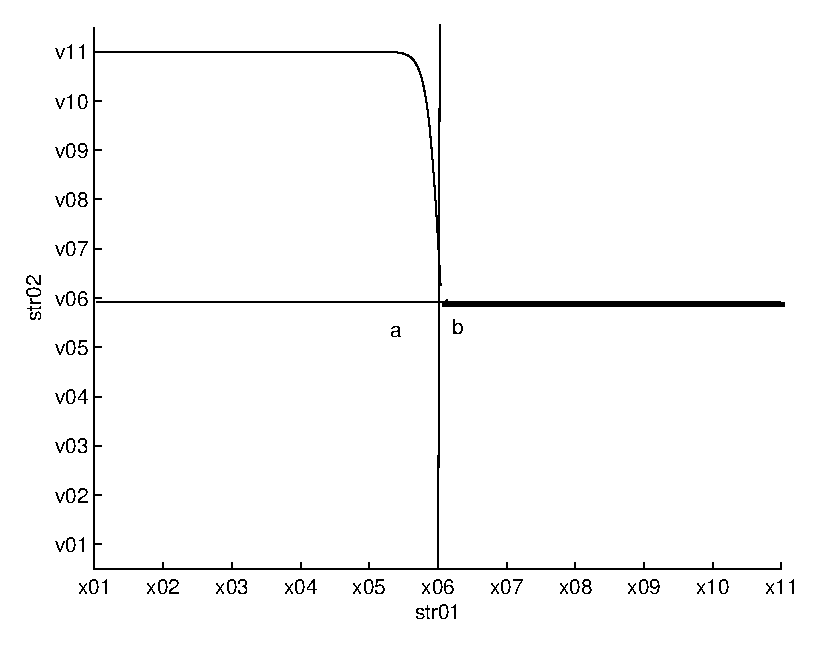
\epsfig{file=./stabilization/eps/subsidy.eps}}%
\end{psfrags}%
%
% End subsidy.tex
\end{figure}\end{document}
% See http://www.uni-kassel.de/~linne/ for recent versions of laprint.m.
%
% created by:           LaPrint version 2.03 (19.1.2000)
% created on:           13-Oct-2009 13:15:05
% options used:         / noextrapicture
% latex width:          12 cm
% factor:               0.8
% eps file name:        subsidy.eps
% eps bounding box:     15 cm x 11.25 cm
% comment:              
%
\begin{psfrags}%
\psfragscanon%
%
% text strings:
\psfrag{str03}[t][t]{x}%
\psfrag{str04}[b][b]{Subsidy factor: $-tanh(x-b)$}%
%
% xticklabels:
\psfrag{x01}[t][t]{-6}%
\psfrag{x02}[t][t]{-4}%
\psfrag{x03}[t][t]{-2}%
\psfrag{x04}[t][t]{0}%
\psfrag{x05}[t][t]{2}%
\psfrag{x06}[t][t]{4}%
\psfrag{x07}[t][t]{6}%
%
% yticklabels:
\psfrag{v01}[r][r]{-1}%
\psfrag{v02}[r][r]{-0.8}%
\psfrag{v03}[r][r]{-0.6}%
\psfrag{v04}[r][r]{-0.4}%
\psfrag{v05}[r][r]{-0.2}%
\psfrag{v06}[r][r]{0}%
\psfrag{v07}[r][r]{0.2}%
\psfrag{v08}[r][r]{0.4}%
\psfrag{v09}[r][r]{0.6}%
\psfrag{v10}[r][r]{0.8}%
\psfrag{v11}[r][r]{1}%
%
% Figure:
\resizebox{12cm}{!}{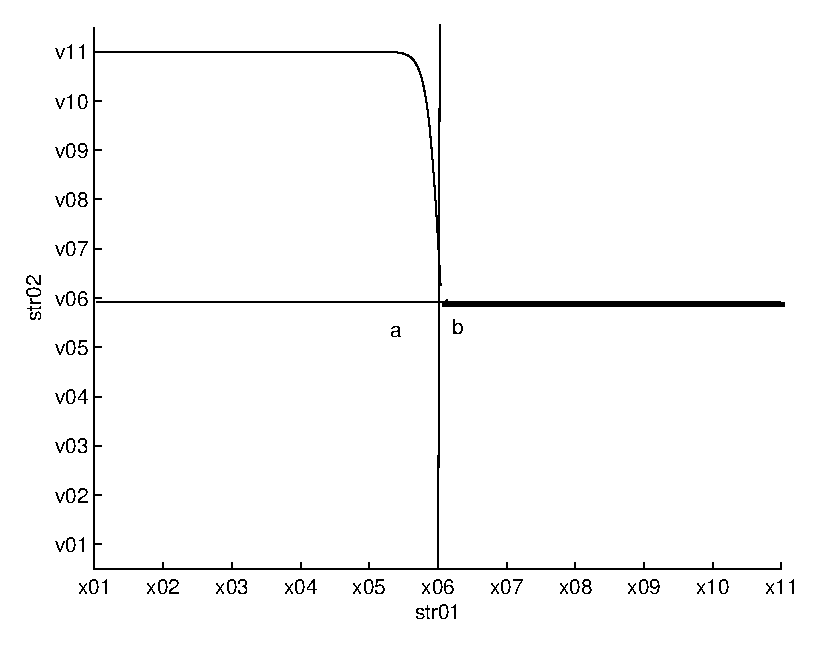
\epsfig{file=./stabilization/eps/subsidy.eps}}%
\end{psfrags}%
%
% End subsidy.tex
\end{figure}\end{document}
% See http://www.uni-kassel.de/~linne/ for recent versions of laprint.m.
%
% created by:           LaPrint version 2.03 (19.1.2000)
% created on:           13-Oct-2009 13:15:05
% options used:         / noextrapicture
% latex width:          12 cm
% factor:               0.8
% eps file name:        subsidy.eps
% eps bounding box:     15 cm x 11.25 cm
% comment:              
%
\begin{psfrags}%
\psfragscanon%
%
% text strings:
\psfrag{str03}[t][t]{x}%
\psfrag{str04}[b][b]{Subsidy factor: $-tanh(x-b)$}%
%
% xticklabels:
\psfrag{x01}[t][t]{-6}%
\psfrag{x02}[t][t]{-4}%
\psfrag{x03}[t][t]{-2}%
\psfrag{x04}[t][t]{0}%
\psfrag{x05}[t][t]{2}%
\psfrag{x06}[t][t]{4}%
\psfrag{x07}[t][t]{6}%
%
% yticklabels:
\psfrag{v01}[r][r]{-1}%
\psfrag{v02}[r][r]{-0.8}%
\psfrag{v03}[r][r]{-0.6}%
\psfrag{v04}[r][r]{-0.4}%
\psfrag{v05}[r][r]{-0.2}%
\psfrag{v06}[r][r]{0}%
\psfrag{v07}[r][r]{0.2}%
\psfrag{v08}[r][r]{0.4}%
\psfrag{v09}[r][r]{0.6}%
\psfrag{v10}[r][r]{0.8}%
\psfrag{v11}[r][r]{1}%
%
% Figure:
\resizebox{12cm}{!}{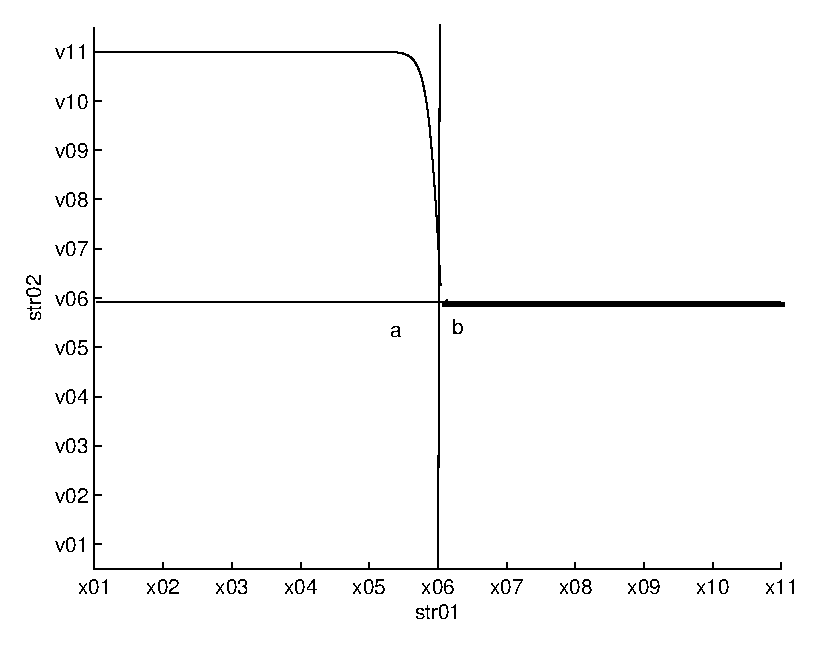
\epsfig{file=./stabilization/eps/subsidy.eps}}%
\end{psfrags}%
%
% End subsidy.tex
}
\end{boxedminipage}
\caption{Graph of the subsidy multiplication factor $s$. To obtain the
actual subsidy this should be multiplied by $|x|$.}
\label{Figure: subsidy multiplication factor}
\end{figure}

In the case of the firm, the subsidy is meant to compensate the firm for an
increase in production costs. These costs consist of labour costs and the
costs of acquiring new capital. Therefore we can use the firm's total
investments as a basis for the subsidy. Firms compute the subsidy amount
truthfully at the end of their subjective month, after they have computed
their capital investments, and send a message to the government informing it
of the amount to be paid.

%\end{document} 